%%%%%%%%%%%%%%%%%%%%%%%%%%%%%%%%%%%%%%%%%%%%%%%%%%%%%%%%%%%%%%%%%%%%%%
% LaTeX Example: Project Report
%
% Source: http://www.howtotex.com
%
% Feel free to distribute this example, but please keep the referral
% to howtotex.com
% Date: March 2011 
% 
%%%%%%%%%%%%%%%%%%%%%%%%%%%%%%%%%%%%%%%%%%%%%%%%%%%%%%%%%%%%%%%%%%%%%%
% How to use writeLaTeX: 
%
% You edit the source code here on the left, and the preview on the
% right shows you the result within a few seconds.
%
% Bookmark this page and share the URL with your co-authors. They can
% edit at the same time!
%
% You can upload figures, bibliographies, custom classes and
% styles using the files menu.
%
% If you're new to LaTeX, the wikibook is a great place to start:
% http://en.wikibooks.org/wiki/LaTeX
%
%%%%%%%%%%%%%%%%%%%%%%%%%%%%%%%%%%%%%%%%%%%%%%%%%%%%%%%%%%%%%%%%%%%%%%
% Edit the title below to update the display in My Documents
%\title{Project Report}
%
%%% Preamble
\documentclass[paper=letter, fontsize=10pt]{scrartcl}
\usepackage[body={7in,7.5in},top=1in, bottom=1in]{geometry}
\usepackage[T1]{fontenc}
\usepackage{fourier}

\usepackage[english]{babel}															% English language/hyphenation
\usepackage[protrusion=true,expansion=true]{microtype}	
\usepackage{amsmath,amsfonts,amsthm} % Math packages
\usepackage[pdftex]{graphicx}	
\usepackage{url}
\usepackage{enumerate}
\usepackage{lastpage}


%%% Custom sectioning
\usepackage{sectsty}
\allsectionsfont{\normalfont\scshape}


%%% Custom headers/footers (fancyhdr package)
\usepackage{fancyhdr}
\usepackage{color,soul}
\pagestyle{fancy}
\fancyhead[L]{}
\fancyhead[c]{Requirements Revision 0}
\fancyhead[R]{\today}											
\fancyfoot[L]{}											 
\fancyfoot[C]{}											
\fancyfoot[R]{\thepage\ of \pageref{LastPage}}		% Pagenumbering
\renewcommand{\headrulewidth}{0.4pt}				% Remove header underlines
\renewcommand{\footrulewidth}{0.4pt}				% Remove footer underlines
\setlength{\headheight}{13.6pt}


%%% Equation and float numbering
\numberwithin{equation}{section}		% Equationnumbering: section.eq#
\numberwithin{figure}{section}			% Figurenumbering: section.fig#
\numberwithin{table}{section}				% Tablenumbering: section.tab#


%%% Maketitle metadata
\newcommand{\horrule}[1]{\rule{\linewidth}{#1}} 	% Horizontal rule
\newcommand{\ts}{\textsuperscript}

%%% Begin document
\begin{document}

\begin{titlepage}

\newcommand{\HRule}{\rule{\linewidth}{0.5mm}} % Defines a new command for the horizontal lines, change thickness here
\newcommand{\authors}{\shortstack{Vitaliy Kondratiev,\\Nathan Johrendt,\\Tyler Lyn,\\Mark Gammie}}

\begin{center}
 
%----------------------------------------------------------------------------------------
%	HEADING SECTIONS
%----------------------------------------------------------------------------------------

\textsc{\LARGE McMaster University}\\[1.5cm] % Name of your university/college
\textsc{\Large CAS 4ZP6}\\[0.5cm]
\textsc{\Large Team 9} \\[0.5cm]
\textsc{\Large Capstone Project 2013/2014}\\[0.5cm] % Major heading such as course name
\textsc{\large Porter Simulation}\\[0.5cm] % Minor heading such as course title

%----------------------------------------------------------------------------------------
%	TITLE SECTION
%----------------------------------------------------------------------------------------

\HRule \\[0.4cm]
{ \huge \bfseries Test Report Revision 0}\\[0.4cm] % Title of your document
\HRule \\[1.5cm]
 
%----------------------------------------------------------------------------------------
%	AUTHOR SECTION
%----------------------------------------------------------------------------------------

\begin{minipage}{0.4\textwidth}
\begin{flushleft} \large
\emph{Authors:}\\
Vitaliy Kondratiev - 0945220\\
Nathan Johrendt - 0950519\\
Tyler Lyn - 0948978\\
Mark Gammie - 0964156
\end{flushleft}
\end{minipage}
~
\begin{minipage}{0.4\textwidth}
\begin{flushright} \large
\emph{Supervisor:} \\
Dr. Douglas Down % Supervisor's Name
\end{flushright}
\end{minipage}\\[4cm]

% If you don't want a supervisor, uncomment the two lines below and remove the section above
%\Large \emph{Author:}\\
%John \textsc{Smith}\\[3cm] % Your name

%----------------------------------------------------------------------------------------
%	DATE SECTION
%----------------------------------------------------------------------------------------

{\large \today}\\[3cm] % Date, change the \today to a set date if you want to be precise

%----------------------------------------------------------------------------------------
%	LOGO SECTION
%----------------------------------------------------------------------------------------

%\includegraphics{Logo}\\[1cm] % Include a department/university logo - this will require the graphicx package
 
%----------------------------------------------------------------------------------------
%Template taken from: http://www.softwaretestinghelp.com/test-plan-sample-softwaretesting-and-quality-assurance-templates/

\vfill % Fill the rest of the page with whitespace
\end{center}
\end{titlepage}

\setcounter{tocdepth}{2}

\tableofcontents

\newpage

\section{Revision History}
\begin{center}
    \begin{tabular}{| c | l | l | l |}
    \hline
    Revision \# & Author & Date & Comment \\ \hline
  	1 & \shortstack{\\Nathan Johrendt} & March 17 & Test Report Template Complete \\ \hline
  	2 & \shortstack{\\Vitaliy Kondratiev,\\Nathan Johrendt,\\Tyler Lyn,\\Mark Gammie} & March 17 & Test Report Updates \\ \hline
  	3 & \shortstack{\\Vitaliy Kondratiev,\\Nathan Johrendt,\\Tyler Lyn,\\Mark Gammie} & March 18 & Test Report Updates \\ \hline
  	4 & \shortstack{\\Vitaliy Kondratiev} & April 12 & Test Report Updates \\ \hline
  	5 & \shortstack{\\Tyler Lyn} & April 16 & Test Report Updates \\ \hline
    \end{tabular}
\end{center}

\section{Introduction}
This testing report is the realization of the test plan written for the Porter Simulation. It contains descriptions and output data for the most important tests from the test plan. The majority of the following test cases are dynamic; many have static versions found within the test plan, but their results are not as valuable, and so they have been omitted.

\section{System Test Reports}
%Specific system tests summarized in terms of initial state, input and expected output. Traceability to requirements and modules
\subsection{Input/Initialization Correctness 1}
The user clicks the Statistical Data File browse button, chooses a file and runs the Simulation. 
\begin{enumerate}[(i)]
	\item \textbf{Initial State:} Uninitialized Simulation   
	\item \textbf{Input:} File path to statistical data file.
	\item \textbf{Expected Results:} After picking a file the user is able to run the simulation 
	\item \textbf{Actual Results on Success:} User is prompted with a file browser. File path is shown after selection. Simulation Starts if the file exists
	\item \textbf{Actual Results on Failure:} User is prompted with a file browser. File path is shown after selection. Simulation does not start. User is prompted with the message "Statistical Data File does not exist" if the file does not exist.
	\item \textbf{Test Results:} Success
\end{enumerate}
	
\subsection{Input/Initialization Correctness 2}
The user clicks the Schedule Data File browse button, chooses a file and runs the Simulation.
\begin{enumerate}[(i)]
	\item \textbf{Initial State:} Uninitialized Simulation   
	\item \textbf{Input:} File path to schedule data file.
	\item \textbf{Expected Results:} After picking the file the user is able to run the simulation
	\item \textbf{Actual Results on Success:} User is prompted with a file browser. File path is shown after selection. Simulation starts if the file exists and is valid
	\item \textbf{Actual Results on Failure I:} User is prompted with a file browser. File path is shown after selection. Simulation does not start if the file does not exist.
	\item \textbf{Actual Results on Failure II:} User is prompted with a file browser. File path is shown after selection. Simulation does not start if the file is not valid. User is prompted with error type and location within file.
		\item \textbf{Test Results:} Success
\end{enumerate}

\subsection{Event List Correctness 1}
As the simulation runs, when a job is dispatched to a porter, it will then have fewer jobs left to assign. This test shows that a Porter is able to take a job and return to a pending state.  Doing this ensures that jobs will be completed and that the event list is correctly moving porters between states. This test involves the simulation core, dispatch and export modules.
\begin{enumerate}[(i)]
	\item \textbf{Initial State:} Simulation event list is generated by sampling the statistical data.
	\item \textbf{Input:} Event list is generated from jobs stored in the data.csv file. The simulation will be configured to add jobs for one day, with 30 porters scheduled 24 hours a day. See Table 3.1: Porter Schedule in schedule.csv below.
	\begin{table}
	\caption{Porter Shift Information in schedule.csv for Event List Correctness 1}
	\begin{center}
    	\begin{tabular}{| c | l | l | l | l |}
    		\hline
        	Shift ID & StartTime & EndTime & Porter Ids & Day \\ \hline
  			0 & 12:00 AM & 11:59 PM & 0,1,2,3,4,5,6,7,8,9,10,11,12,13,14,15,16,17,18,19,20,21,22,23,24,25,26,27,28,29 & 0 \\ \hline
  			1 & 12:00 AM & 11:59 PM & 0,1,2,3,4,5,6,7,8,9,10,11,12,13,14,15,16,17,18,19,20,21,22,23,24,25,26,27,28,29 & 1 \\ \hline
  			2 & 12:00 AM & 11:59 PM & 0,1,2,3,4,5,6,7,8,9,10,11,12,13,14,15,16,17,18,19,20,21,22,23,24,25,26,27,28,29 & 2 \\ \hline
  			3 & 12:00 AM & 11:59 PM & 0,1,2,3,4,5,6,7,8,9,10,11,12,13,14,15,16,17,18,19,20,21,22,23,24,25,26,27,28,29 & 3 \\ \hline
  			4 & 12:00 AM & 11:59 PM & 0,1,2,3,4,5,6,7,8,9,10,11,12,13,14,15,16,17,18,19,20,21,22,23,24,25,26,27,28,29 & 4 \\ \hline
  			5 & 12:00 AM & 11:59 PM & 0,1,2,3,4,5,6,7,8,9,10,11,12,13,14,15,16,17,18,19,20,21,22,23,24,25,26,27,28,29 & 5 \\ \hline
  			6 & 12:00 AM & 11:59 PM & 0,1,2,3,4,5,6,7,8,9,10,11,12,13,14,15,16,17,18,19,20,21,22,23,24,25,26,27,28,29 & 6 \\ \hline
    	\end{tabular}
	\end{center}
	\end{table}
	\item \textbf{Expected Output:} Conclude that no incomplete jobs remain
	\item \textbf{Actual Output:} \\
Porter1 is complete Job203: Emergency Department Bed 02 -> E2 Orthopedics (3502)\\
Porter8 is complete Job198: F5 ALC Room 12 Bed 01 -> X-Ray Core - B1 (2245)\\
\hl{Porter6 is dispatched Job206: X-Ray Core - B1 (2245) -> F5 ALC Room 05 Bed 03}\\
Porter8 is pending\\
Porter0 is complete Job201: F5 ALC Room 05 Bed 03 -> X-Ray Core - B1 (2245)\\
\hl{Porter6 is in-progress Job206: X-Ray Core - B1 (2245) -> F5 ALC Room 05 Bed 03}\\
Porter2 is complete Job205: Emergency Department Bed 04 -> E2 Orthopedics (3502)\\
\hl{Porter6 is complete Job206: X-Ray Core - B1 (2245) -> F5 ALC Room 05 Bed 03}\\
Porter0 is pending\\
Porter10 is complete Job191: F3 Medicine Room 14 Bed 04 -> E3 Medicine Room 11 Bed 01\\
Porter2 is pending\\
Porter10 is pending\\
Porter3 is complete Job202: C3 Oncology Room 24 Bed 01 -> Morgue (2032)\\
Porter1 is pending\\
\hl{Porter6 is pending}\\
Porter3 is pending\\
Porter10 is dispatched Job204: Emergency Department Bed 04 -> E2 Orthopedics (3502)\\
Porter10 is in-progress Job204: Emergency Department Bed 04 -> E2 Orthopedics (3502)\\
*****SIMULATION COMPLETE*****
	\item \textbf{Test Results:} Success
\end{enumerate}

\subsection{State Change Correctness 1}
Porters will be required to change state frequently as they complete all of a regular day's tasks understaffed. Any problems, beyond the obvious delays, will result in a Porter getting stuck with a job at a particular state. This will be recorded in the output data and can be addressed.  This test ensures that  the porters return to the pending state unless the Simulation has finished.
\begin{enumerate}[(i)]
	\item \textbf{Initial State:} Simulation event list is generated by initializing the simulation through the interface
	\item \textbf{Input:} Event list is generated from jobs stored in the data.csv file. Porter schedule is generated from the schedule.csv file. The simulation will be configured to add jobs for one day, with five porters scheduled 24 hours that day.
	\begin{table}
	\caption{Porter Shift Information in schedule.csv for State Change Correctness 1}
	\begin{center}
    	\begin{tabular}{| c | l | l | l | l |}
    		\hline
        	Shift ID & StartTime & EndTime & Porter Ids & Day \\ \hline
  			0 & 12:00 AM & 11:59 PM & 0,1,2,3,4,6,7,8,9,10 & 0 \\ \hline
    	\end{tabular}
	\end{center}
	\end{table}
	\item \textbf{Expected Output:} All Porters complete jobs dispatched to them successfully until the simulation duration expires
	\item \textbf{Actual Output:}\\
Porter1 is complete Job203: Emergency Department Bed 02 -> E2 Orthopedics (3502)\\
Porter8 is complete Job198: F5 ALC Room 12 Bed 01 -> X-Ray Core - B1 (2245)\\
Porter6 is dispatched Job206: X-Ray Core - B1 (2245) -> F5 ALC Room 05 Bed 03\\
Porter8 is pending\\
Porter0 is complete Job201: F5 ALC Room 05 Bed 03 -> X-Ray Core - B1 (2245)\\
Porter6 is in-progress Job206: X-Ray Core - B1 (2245) -> F5 ALC Room 05 Bed 03\\
Porter2 is complete Job205: Emergency Department Bed 04 -> E2 Orthopedics (3502)\\
Porter6 is complete Job206: X-Ray Core - B1 (2245) -> F5 ALC Room 05 Bed 03\\
Porter0 is pending\\
Porter10 is complete Job191: F3 Medicine Room 14 Bed 04 -> E3 Medicine Room 11 Bed 01\\
Porter2 is pending\\
Porter10 is pending\\
Porter3 is complete Job202: C3 Oncology Room 24 Bed 01 -> Morgue (2032)\\
Porter1 is pending\\
Porter6 is pending\\
Porter3 is pending\\
\hl{Porter10 is dispatched Job204: Emergency Department Bed 04 -> E2 Orthopedics (3502)}\\
\hl{Porter10 is in-progress Job204: Emergency Department Bed 04 -> E2 Orthopedics (3502)}\\
*****SIMULATION COMPLETE*****\\

	\item \textbf{Test Results:} Success
\end{enumerate}

\subsection{State Change Correctness 3}
\begin{enumerate}[(i)]
		\item \textbf{Initial State:} Initialized simulation
		\item \textbf{Input:} porterUnit.py unit testing file
		\item \textbf{Description:} Through the use of UnitTest in python, this test checks that a porter starts in a pending state and is able to iterates through all states when a porter is given a job.
		\item \textbf{Expected Output:} The porter is in the pending state after work is complete.
		\item \textbf{Actual Output:} Run the python module: python porterUnit.py\\
.\\
----------------------------------------------------------------------\\
Ran 1 test in 0.001s\\

OK
\end{enumerate}

\subsection{Porter/Event Linkage Correctness 1}
Every time an Event moves from pending to dispatched, a Porter must be linked to that event. This test is to ensure that all pairings of job and Porter are unique, and that after completing a job, a porter will return to "available" and continue accepting new jobs. This test involves the simulation core, dispatch and export modules.
\begin{enumerate}[(i)]
	\item \textbf{Initial State:} Simulation event list and porter schedule are generated by initializing the simulation through the interface
	\item \textbf{Input:} Event list is generated from jobs stored in the data.csv file. Porter schedule is generated from the schedule.csv file. The simulation will be configured to add jobs for one day, with 30 porters scheduled 24 hours that day.
	\begin{table}
	\caption{Porter Shift Information in schedule.csv for Porter/Event Linkage Correctness 1}
	\begin{center}
    	\begin{tabular}{| c | l | l | l | l |}
    		\hline
        	Shift ID & StartTime & EndTime & Porter Ids & Day \\ \hline
  			0 & 12:00 AM & 11:59 PM & 0,1,2,3,4,5,6,7,8,9,10,11,12,13,14,15,16,17,18,19,20,21,22,23,24,25,26,27,28,29 & 0 \\ \hline
    	\end{tabular}
	\end{center}
	\end{table}
	\item \textbf{Expected Output:} Porter and Event are linked together uniquely
	\item \textbf{Actual Output:} 
Porter23 is complete Job13: CDU Express Bed 05 -> Ultrasound (2276)\\
Porter17 is pending\\
Porter27 is complete Job12: E3 Medicine Room 02 Bed 01 -> Ultrasound (2276)\\
Porter21 is pending\\
Porter26 is pending\\
Porter24 is pending\\
Porter28 is complete Job18: CT - B1 (3023) -> E3 Medicine Room 01 Bed 01
Porter25 is complete Job26: Ultrasound (2276) -> E3 Medicine Room 02 Bed 01
Porter23 is pending\\
Porter29 is complete Job24: Ultrasound (2276) -> CDU Express Bed 05
Porter27 is pending\\
Porter25 is pending\\
Porter28 is pending\\
Porter29 is pending\\
*****SIMULATION COMPLETE*****\\
	\item \textbf{Test Results:} Success
\end{enumerate}

\subsection{Task Pool Correctness 1}
With only a single porter active, the majority of the jobs added by the simulation will simply be added to the dispatcher and wait. This test is to ensure that the dispatcher holds incomplete jobs correctly and that they are reported after the simulation completes. This test involves the simulation core, dispatch and export modules.
\begin{enumerate}[(i)]
	\item \textbf{Initial State:} Simulation event list and porter schedule are generated by initializing the simulation through the interface
	\item \textbf{Input:} Event list is generated from jobs stored in the data.csv file. Porter schedule is generated from the schedule.csv file. The simulation will be configured to add jobs for one day, with one Porter scheduled 24 hours a day.
	\begin{table}
	\caption{Porter Shift Information in schedule.csv for Task Pool Correctness 1}
	\begin{center}
    	\begin{tabular}{| c | l | l | l | l |}
    		\hline
        	Shift ID & StartTime & EndTime & Porter Ids & Day \\ \hline
  			0 & 12:00 AM & 11:59 PM & 0 & 0 \\ \hline
    	\end{tabular}
	\end{center}
	\end{table}
	\item \textbf{Expected Output:} Simulation output properly stores many incomplete job entries.
	\item \textbf{Actual Output:} \\
Porter0 is pending\\
Porter0 is dispatched Job67: Ultrasound (2276) -> CDU Express Bed 02\\
Porter0 is in-progress Job67: Ultrasound (2276) -> CDU Express Bed 02\\
Porter0 is complete Job67: Ultrasound (2276) -> CDU Express Bed 02\\
Porter0 is pending\\
Porter0 is dispatched Job50: C3 Oncology Room 23 Bed 01 -> JC 21H (3747)\\
Porter0 is in-progress Job50: C3 Oncology Room 23 Bed 01 -> JC 21H (3747)\\
Porter0 is complete Job50: C3 Oncology Room 23 Bed 01 -> JC 21H (3747)\\
Porter0 is pending\\
Porter0 is dispatched Job41: MSR Ward 3 Rehab Room 15 Bed 01 -> CT - B1 (3023)\\
Porter0 is in-progress Job41: MSR Ward 3 Rehab Room 15 Bed 01 -> CT - B1 (3023)\\
Porter0 is complete Job41: MSR Ward 3 Rehab Room 15 Bed 01 -> CT - B1 (3023)\\
Porter0 is pending\\
Porter0 is dispatched Job33: C3 Oncology/GI Medicine Nurse (3395) -> JC Clinic B (3620)\\
Porter0 is in-progress Job33: C3 Oncology/GI Medicine Nurse (3395) -> JC Clinic B (3620)\\
Porter0 is complete Job33: C3 Oncology/GI Medicine Nurse (3395) -> JC Clinic B (3620)\\
Porter0 is pending\\
Porter0 is dispatched Job60: DI Intervention \#1 (2274) -> Endoscopy (2334)\\
Porter0 is in-progress Job60: DI Intervention \#1 (2274) -> Endoscopy (2334)\\
Porter0 is complete Job60: DI Intervention \#1 (2274) -> Endoscopy (2334)\\
Porter0 is pending\\
Porter0 is dispatched Job28: E4 Room 07 Bed 01 -> CT - B1 (3023)\\
*****SIMULATION COMPLETE*****\\
	\item \textbf{Test Results:} Success
\end{enumerate}

\subsection{Task Pool Correctness 3}
Through the use of UnitTest in python, this test checks that the dispatcher correctly adds a new job to the Task Pool if there are no available Porters. Three specific variables are tested for: Priority Weight, Appointment Factor and the length of the pending jobs list. This test deals exclusively with the dispatcher module.
\begin{enumerate}[(i)]
	\item \textbf{Initial State:} Initialized simulation
	\item \textbf{Input:} dispatcherUnit.py unit testing file %Could include source code here
	\item \textbf{Expected Output:} Conclude that the Task Pool contains one additional event as the number of pending jobs has increased by one.
	\item \textbf{Actual Output:} Run the python module: python dispatcherUnit.py\\
...\\
----------------------------------------------------------------------\\
Ran 3 tests in 0.003s\\

OK
\end{enumerate}

\subsection{Termination Correctness 1}
After accepting all inputs and initializing, the simulation will compute five days of operational data and output the results. This test involves all modules.
\begin{enumerate}[(i)]
	\item \textbf{Initial State:} Simulation is initialized through the interface
	\item \textbf{Input:} Event list is generated from jobs stored in the data.csv file. Porter schedule is generated from the schedule.csv file. The simulation will be configured to add jobs for five days, with 30 porters scheduled 24 hours a day.
	\begin{table}
	\caption{Porter Shift Information in schedule.csv for Termination Correctness 1}
	\begin{center}
    	\begin{tabular}{| c | l | l | l | l |}
    		\hline
        	Shift ID & StartTime & EndTime & Porter Ids & Day \\ \hline
  			0 & 12:00 AM & 11:59 PM & 0,1,2,3,4,5,6,7,8,9,10,11,12,13,14,15,16,17,18,19,20,21,22,23,24,25,26,27,28,29 & 0 \\ \hline
  			1 & 12:00 AM & 11:59 PM & 0,1,2,3,4,5,6,7,8,9,10,11,12,13,14,15,16,17,18,19,20,21,22,23,24,25,26,27,28,29 & 1 \\ \hline
  			2 & 12:00 AM & 11:59 PM & 0,1,2,3,4,5,6,7,8,9,10,11,12,13,14,15,16,17,18,19,20,21,22,23,24,25,26,27,28,29 & 2 \\ \hline
  			3 & 12:00 AM & 11:59 PM & 0,1,2,3,4,5,6,7,8,9,10,11,12,13,14,15,16,17,18,19,20,21,22,23,24,25,26,27,28,29 & 3 \\ \hline
  			4 & 12:00 AM & 11:59 PM & 0,1,2,3,4,5,6,7,8,9,10,11,12,13,14,15,16,17,18,19,20,21,22,23,24,25,26,27,28,29 & 4 \\ \hline
  			5 & 12:00 AM & 11:59 PM & 0,1,2,3,4,5,6,7,8,9,10,11,12,13,14,15,16,17,18,19,20,21,22,23,24,25,26,27,28,29 & 5 \\ \hline
  			6 & 12:00 AM & 11:59 PM & 0,1,2,3,4,5,6,7,8,9,10,11,12,13,14,15,16,17,18,19,20,21,22,23,24,25,26,27,28,29 & 6 \\ \hline
    	\end{tabular}
	\end{center}
	\end{table}
	\item \textbf{Expected Output:} Simulation outputs that it has completed each step and has written the results to the dashboard.
	\item \textbf{Actual Output:}\\
	*****SIMULATION COMPLETE*****\\
	*****WRITING OUTPUT*****\\
	*****SAVING OUTPUT*****\\
	*****BUILDING DASHBOARD*****\\
	*****DASHBOARD COMPLETE*****\\
	\item textbf{Test Results:} Success
\end{enumerate}

\subsection{Compatibility Test 1} %add info for cxfreeze
The simulation is run and compared to results computed on other operating systems to ensure it is functioning normally in the new environment. The stakeholders have indicated that they will only be using the software on versions of windows. The current implementation utilizes cxfreeze to create windows executable files. 
\begin{enumerate}[(i)]
	\item \textbf{Initial State:} Unknown Operating System with the simulation accessible on local storage
	\item \textbf{Input:} 'Termination Correctness 1' simulation parameters (details outline previously under 'Termination Correctness 1')
	\item \textbf{Expected Output:} Simulated results are consistent with previously generated values
	\item \textbf{Actual Output:} Currently, the simulation has been tested on a number of systems, including windows 7 and 8, and the executables produced by cxfreeze have performed perfectly. Final output from each simulation compatibility test has been: \\
	*****SIMULATION COMPLETE*****\\
	*****WRITING OUTPUT*****\\
	*****SAVING OUTPUT*****\\
	*****BUILDING DASHBOARD*****\\
	*****DASHBOARD COMPLETE*****\\
	\item textbf{Test Results:} Success
\end{enumerate}

\section{Nonfunctional Test Reports}
\subsection{Usability Test 1}
End user is provided with a set of instructions from the user manual on how to initialize and run the simulation. The success of this test is determined by how much external assistance the End User requires from the development team on their first use of the software. 
\begin{enumerate}[(i)]
	\item \textbf{Initial State:} Simulation prior to execution
	\item \textbf{Input:} End user with a copy of both the simulation software package and accompanying user manual.
	\item \textbf{Expected Output:} The end user successfully Initializes the Simulation
	\item \textbf{Actual Output:} The simulation is yet to be formally tested with stakeholders in regards to the scope of this test case. However, feedback has been gathered during project demos with a few key stakeholders, and the responses have been positive. This test will become critical during the very final stages of development, as the interface for the project is being tailored to the stakeholder's needs.
\end{enumerate}

\subsection{Performance Test 1}
The project stakeholders have placed a loose time limit on the duration of execution for a single simulation run of fifteen minutes. No correct simulation execution has taken longer than five minutes, with most between one and two minutes, but ensuring this general timing for the simulation across all applicable systems is the purpose of this test.
\begin{enumerate}[(i)]
	\item \textbf{Initial State:} Simulation prior to execution 
	\item \textbf{Input:} Any combination of inputs that the interface will accept and begin simulating
	\item \textbf{Expected Output:} The simulation completes execution taking between thirty seconds and five minutes, repeated thrice for consistency.
	\item \textbf{Actual Output:}
	\begin{table}
	\caption{Simulation Execution Times for Performance Test 1}
	\begin{center}
    	\begin{tabular}{| c | c | c |}
    		\hline
        	Simulation Run & Simulation Period (\# of days) & Duration of Execution (seconds) \\ \hline
  			1 & 1 & 19.945 \\ \hline
  			2 & 1 & 21.861 \\ \hline
  			3 & 1 & 20.442 \\ \hline
  			4 & 2 & 25.713 \\ \hline
  			5 & 2 & 22.823 \\ \hline
  			6 & 2 & 22.592 \\ \hline
  			7 & 3 & 25.569 \\ \hline
  			8 & 3 & 28.569 \\ \hline
  			9 & 3 & 26.850 \\ \hline
  			10 & 4 & 33.673 \\ \hline
  			11 & 4 & 32.964 \\ \hline
  			12 & 4 & 32.206 \\ \hline
  			13 & 5 & 39.469 \\ \hline
  			14 & 5 & 39.942 \\ \hline
  			15 & 5 & 39.157 \\ \hline
    	\end{tabular}
	\end{center}
	\end{table}
		
\end{enumerate}

	\begin{figure}[!htbp]
		\begin{center}
			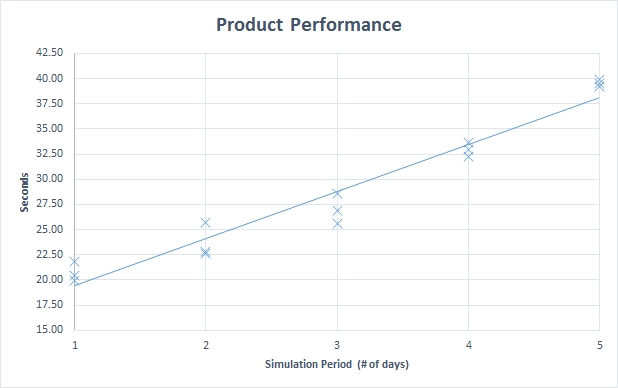
\includegraphics[width=1\columnwidth, height=0.4\textheight, keepaspectratio] {performancereport.png}
			\caption{Performance Report}
		\end{center}
	\end{figure}

\section{Summary}
%Changes made as a result of testing, talk about automated testing
Over the past few weeks, our implementation has been dramatically overhauled, resulting in brand new methods for importing and information handling. At the current state of development, the previously defined automated testing techniques were no longer applicable, and have been omitted from this report. Approaching the final implementation, the project team anticipates that a number of automated tests will be re-added to the test plan and report. 
\\
These test cases, whether performed as a formal testing suite or quick samples during implementation changes, have provided useful information for repairing or improving the simulation software. Many of these tests have produced expected results without fail, but they provide essential security by repeatedly checking the core features of the software, ensuring accuracy throughout development.   One test in particular, Task Pool Correctness 1, which overloads a single porter with many tasks to test the dispatcher's ability to store pending jobs, highlighted a major problem with how jobs were dispatched. Jobs from the beginning of a day weren't being handled by a porter until the very end, this led to an examination of the dispatcher module and the resolution of the issue. 
\section{Figures and Tables Appendix}
\begin{enumerate}[(a)]
	\item Figure 3.1: User Interface
	\item Table  3.1: Porter Shift Information in schedule.csv for Event List Correctness 1
	\item Table  3.2: Porter Shift Information in schedule.csv for State Change Correctness 1
	\item Table  3.3: Porter Shift Information in schedule.csv for Porter/Event Linkage Correctness 1
	\item Table  3.4: Porter Shift Information in schedule.csv for Task Pool Correctness 1
	\item Table  3.5: Porter Shift Information in schedule.csv for Termination Correctness 1
	\item Table  4.1: Simulation Execution Times for Performance Test 1
	\item Figure 4.1: Performance Report
\end{enumerate}

%%% End document
\end{document}